\makeatletter\def\input@path{{minimus}{standalone-silicon}}\makeatother

\documentclass{standalone-silicon}

\usepackage{minimus-text}
\usepackage{minimus-math}
\usepackage{minimus-tikz}

\begin{document}
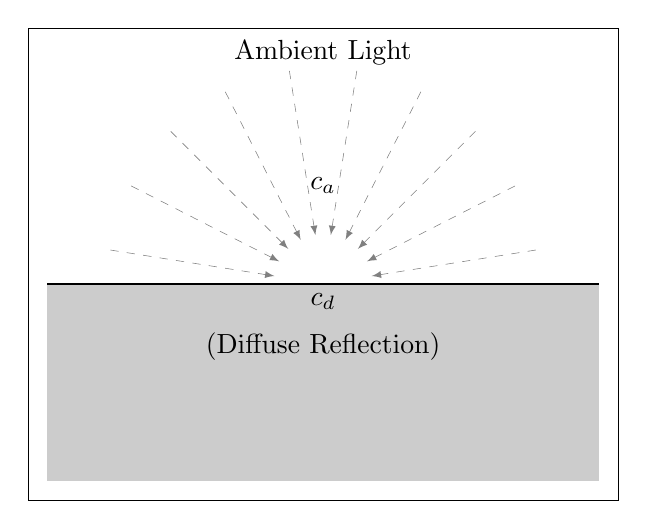
\begin{tikzpicture}[scale=1.25]

\fill[black!20!white] (-2.8,0) rectangle (2.8,-2);
\draw[thick] (-2.8,0) -- (2.8,0);

\path (0,0) coordinate (O) node[below] {$c_d$} node[below=0.5cm] {(Diffuse Reflection)};

\path (0,2.35) node {Ambient Light};
\path (0,1) node {$c_a$};

\foreach \x in {9,27,...,171}
{
    \draw[very thin,latex-,gray,dashed]  (\x:0.5) -- (\x:2.25);
}

\draw[ultra thin] (-3,-2.2) rectangle (3,2.6);

\end{tikzpicture}
\end{document}